\section{Architecture}
In \autoref{arch}, a broad overview of the architecture of the application is given. We use the global mode for all the services in docker swarm mode, which means that all of these services are represented at each of the nodes in the cluster.

    \begin{figure}[H]
		\centering
		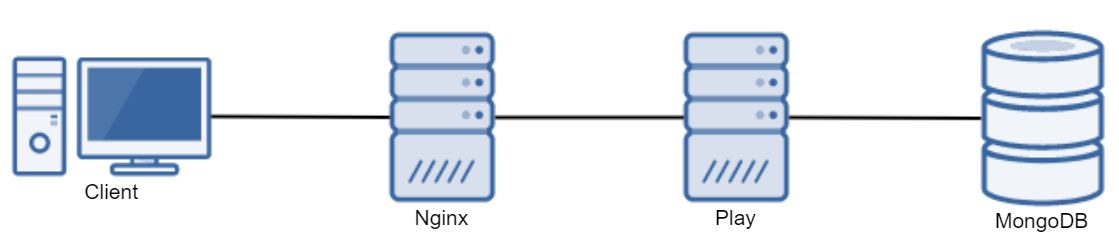
\includegraphics[width=1.0\textwidth]{images/Architecture.png}
		\caption{Overview of the architecture of Uber for Bikes}
		\label{arch}
	\end{figure}
	
For our webserver we have written the main component in Scala. Scala is a functional programming language supporting high scalability. We used the Play framework which fits our purposes very well as it is designed for developing web applications.  As well as this, it ensures the integration with the database through the corresponding driver. 

For our project we used the MongoDB database with a ReactiveMongo driver. ReactiveMongo is a Scala driver that provides fully non-blocking and asynchronous I/O operations. ReactiveMongo is designed to avoid any kind of blocking request. Every operation returns immediately, freeing the running thread and resuming execution when it is over.

In the frond-end, AngularJS and Bootstrap are used for providing a nice user interface. The UI serves a simple purpose: Renting and unrenting bikes. The main view of the UI is a Google Maps view. It is currently set to the location of Groningen, but could eventually be used to show the region where the user resides.
In our project we use an external third party service. The service of Google is needed to enable the conversion between a textual representation of a location and the corresponding geographical representation of the GPS system. This conversion is done via the Google Maps API.


\subsection{Docker swarm}

Docker swarm is a tool that enables high scalability and fault-tolerance. With Docker swarm, it is possible to run applications on a cluster of virtual or physical machines. If one of the nodes or one of the containers fails the other keep functioning, which provides high fault tolerance. The scalability can be controlled easily as well. For every service, there are two modes available, global and replicated. If  the replicated mode is used, the user can define the number of replicas of each container. After that, they are distributed among all the nodes of the cluster. If the global mode is used, every node in the cluster runs exactly one instance of the service. In our application, we use global mode for all the services except one (see \ref{db_disc}), which means that if we run our application on two (virtual) machines, each machine will always have exactly one instance of every service running on it.
